%  LaTeX support: latex@mdpi.com 
%  For support, please attach all files needed for compiling as well as the log file, and specify your operating system, LaTeX version, and LaTeX editor.

%=================================================================
\documentclass[entropy,article,submit,pdftex,moreauthors]{Definitions/mdpi} 

%--------------------
% Class Options:
%--------------------
%----------
% journal
%----------
% Choose between the following MDPI journals:
% acoustics, actuators, addictions, admsci, adolescents, aerobiology, aerospace, agriculture, agriengineering, agrochemicals, agronomy, ai, air, algorithms, allergies, alloys, analytica, analytics, anatomia, animals, antibiotics, antibodies, antioxidants, applbiosci, appliedchem, appliedmath, applmech, applmicrobiol, applnano, applsci, aquacj, architecture, arm, arthropoda, arts, asc, asi, astronomy, atmosphere, atoms, audiolres, automation, axioms, bacteria, batteries, bdcc, behavsci, beverages, biochem, bioengineering, biologics, biology, biomass, biomechanics, biomed, biomedicines, biomedinformatics, biomimetics, biomolecules, biophysica, biosensors, biotech, birds, bloods, blsf, brainsci, breath, buildings, businesses, cancers, carbon, cardiogenetics, catalysts, cells, ceramics, challenges, chemengineering, chemistry, chemosensors, chemproc, children, chips, cimb, civileng, cleantechnol, climate, clinpract, clockssleep, cmd, coasts, coatings, colloids, colorants, commodities, compounds, computation, computers, condensedmatter, conservation, constrmater, cosmetics, covid, crops, cryptography, crystals, csmf, ctn, curroncol, cyber, dairy, data, ddc, dentistry, dermato, dermatopathology, designs, devices, diabetology, diagnostics, dietetics, digital, disabilities, diseases, diversity, dna, drones, dynamics, earth, ebj, ecologies, econometrics, economies, education, ejihpe, electricity, electrochem, electronicmat, electronics, encyclopedia, endocrines, energies, eng, engproc, entomology, entropy, environments, environsciproc, epidemiologia, epigenomes, est, fermentation, fibers, fintech, fire, fishes, fluids, foods, forecasting, forensicsci, forests, foundations, fractalfract, fuels, future, futureinternet, futurepharmacol, futurephys, futuretransp, galaxies, games, gases, gastroent, gastrointestdisord, gels, genealogy, genes, geographies, geohazards, geomatics, geosciences, geotechnics, geriatrics, grasses, gucdd, hazardousmatters, healthcare, hearts, hemato, hematolrep, heritage, higheredu, highthroughput, histories, horticulturae, hospitals, humanities, humans, hydrobiology, hydrogen, hydrology, hygiene, idr, ijerph, ijfs, ijgi, ijms, ijns, ijpb, ijtm, ijtpp, ime, immuno, informatics, information, infrastructures, inorganics, insects, instruments, inventions, iot, j, jal, jcdd, jcm, jcp, jcs, jcto, jdb, jeta, jfb, jfmk, jimaging, jintelligence, jlpea, jmmp, jmp, jmse, jne, jnt, jof, joitmc, jor, journalmedia, jox, jpm, jrfm, jsan, jtaer, jvd, jzbg, kidneydial, kinasesphosphatases, knowledge, land, languages, laws, life, liquids, literature, livers, logics, logistics, lubricants, lymphatics, machines, macromol, magnetism, magnetochemistry, make, marinedrugs, materials, materproc, mathematics, mca, measurements, medicina, medicines, medsci, membranes, merits, metabolites, metals, meteorology, methane, metrology, micro, microarrays, microbiolres, micromachines, microorganisms, microplastics, minerals, mining, modelling, molbank, molecules, mps, msf, mti, muscles, nanoenergyadv, nanomanufacturing,\gdef\@continuouspages{yes}} nanomaterials, ncrna, ndt, network, neuroglia, neurolint, neurosci, nitrogen, notspecified, %%nri, nursrep, nutraceuticals, nutrients, obesities, oceans, ohbm, onco, %oncopathology, optics, oral, organics, organoids, osteology, oxygen, parasites, parasitologia, particles, pathogens, pathophysiology, pediatrrep, pharmaceuticals, pharmaceutics, pharmacoepidemiology,\gdef\@ISSN{2813-0618}\gdef\@continuous pharmacy, philosophies, photochem, photonics, phycology, physchem, physics, physiologia, plants, plasma, platforms, pollutants, polymers, polysaccharides, poultry, powders, preprints, proceedings, processes, prosthesis, proteomes, psf, psych, psychiatryint, psychoactives, publications, quantumrep, quaternary, qubs, radiation, reactions, receptors, recycling, regeneration, religions, remotesensing, reports, reprodmed, resources, rheumato, risks, robotics, ruminants, safety, sci, scipharm, sclerosis, seeds, sensors, separations, sexes, signals, sinusitis, skins, smartcities, sna, societies, socsci, software, soilsystems, solar, solids, spectroscj, sports, standards, stats, std, stresses, surfaces, surgeries, suschem, sustainability, symmetry, synbio, systems, targets, taxonomy, technologies, telecom, test, textiles, thalassrep, thermo, tomography, tourismhosp, toxics, toxins, transplantology, transportation, traumacare, traumas, tropicalmed, universe, urbansci, uro, vaccines, vehicles, venereology, vetsci, vibration, virtualworlds, viruses, vision, waste, water, wem, wevj, wind, women, world, youth, zoonoticdis 
% For posting an early version of this manuscript as a preprint, you may use "preprints" as the journal. Changing "submit" to "accept" before posting will remove line numbers.

%---------
% article
%---------
% The default type of manuscript is "article", but can be replaced by: 
% abstract, addendum, article, book, bookreview, briefreport, casereport, comment, commentary, communication, conferenceproceedings, correction, conferencereport, entry, expressionofconcern, extendedabstract, datadescriptor, editorial, essay, erratum, hypothesis, interestingimage, obituary, opinion, projectreport, reply, retraction, review, perspective, protocol, shortnote, studyprotocol, systematicreview, supfile, technicalnote, viewpoint, guidelines, registeredreport, tutorial
% supfile = supplementary materials

%----------
% submit
%----------
% The class option "submit" will be changed to "accept" by the Editorial Office when the paper is accepted. This will only make changes to the frontpage (e.g., the logo of the journal will get visible), the headings, and the copyright information. Also, line numbering will be removed. Journal info and pagination for accepted papers will also be assigned by the Editorial Office.

%------------------
% moreauthors
%------------------
% If there is only one author the class option oneauthor should be used. Otherwise use the class option moreauthors.

%---------
% pdftex
%---------
% The option pdftex is for use with pdfLaTeX. Remove "pdftex" for (1) compiling with LaTeX & dvi2pdf (if eps figures are used) or for (2) compiling with XeLaTeX.

\bibliographystyle{apsrev4-2}

%=================================================================
% MDPI internal commands - do not modify
\firstpage{1} 
\makeatletter 
\setcounter{page}{\@firstpage} 
\makeatother
\pubvolume{1}
\issuenum{1}
\articlenumber{0}
\pubyear{2024}
\copyrightyear{2024}
%\externaleditor{Academic Editor: Firstname Lastname}
\datereceived{ } 
\daterevised{ } % Comment out if no revised date
\dateaccepted{ } 
\datepublished{ } 
%\datecorrected{} % For corrected papers: "Corrected: XXX" date in the original paper.
%\dateretracted{} % For corrected papers: "Retracted: XXX" date in the original paper.
\hreflink{https://doi.org/} % If needed use \linebreak
%\doinum{}
%\pdfoutput=1 % Uncommented for upload to arXiv.org
%\CorrStatement{yes}  % For updates


%=================================================================
% Add packages and commands here. The following packages are loaded in our class file: fontenc, inputenc, calc, indentfirst, fancyhdr, graphicx, epstopdf, lastpage, ifthen, float, amsmath, amssymb, lineno, setspace, enumitem, mathpazo, booktabs, titlesec, etoolbox, tabto, xcolor, colortbl, soul, multirow, microtype, tikz, totcount, changepage, attrib, upgreek, array, tabularx, pbox, ragged2e, tocloft, marginnote, marginfix, enotez, amsthm, natbib, hyperref, cleveref, scrextend, url, geometry, newfloat, caption, draftwatermark, seqsplit
% cleveref: load \crefname definitions after \begin{document}

\usepackage{amsmath,amssymb,amsbsy,txfonts}
\usepackage{bbm,times}
\usepackage[T1]{fontenc}
\usepackage{braket}
\usepackage{epsfig} 

\usepackage{graphicx}% Include figure files
\usepackage{dcolumn}% Align table columns on decimal point
\usepackage{bm}% bold math
%\usepackage{ulem}

\usepackage{physics}
\usepackage{xcolor}

%\usepackage{hyperref}% add hypertext capabilities
%\usepackage{cleveref}
%\hypersetup{colorlinks=true, linkcolor=blue}

\providecommand{\openone}{\leavevmode\hbox{\small1\kern-3.8pt\normalsize1}}

\usepackage{soul}
\usepackage{cancel}
\usepackage{float}
\usepackage{multirow}
\newcolumntype{?}{!{\vrule width 1.8pt}}

\usepackage{colortbl}

\graphicspath{{images/}}

% Custom commands
\renewcommand{\a}{\hat{a}}
\newcommand{\ad}{\hat{a}^\dagger}
\renewcommand{\b}{\hat{b}}
\newcommand{\bd}{\hat{b}^\dagger}
\newcommand{\opV}[1][k]{\hat{V}_{#1}}
\newcommand{\opU}[1][k]{\hat{U}_{#1}}
\newcommand{\ops}[2]{\hat{\sigma}_#1^#2}
\newcommand{\opsup}[1]{\dyad{e}{g#1}}
\newcommand{\opsdwn}[1]{\dyad{g#1}{e}}
\renewcommand{\tt}{\theta^2}
\newcommand{\dissipator}[1][n]{\mathcal{D}_S[\rho_{#1}]}
\newcommand{\ga}{\gamma_\alpha}
\newcommand{\gb}{\gamma_\beta}
\newcommand{\idd}{\mathbb{I}}
\newcommand{\C}{\hat{C}}
\newcommand{\Cp}{\hat{C}'}
\newcommand{\Sd}{\hat{S}^\dagger}
\renewcommand{\S}{\hat{S}}
\renewcommand{\r}{\rho}


%=================================================================
% Please use the following mathematics environments: Theorem, Lemma, Corollary, Proposition, Characterization, Property, Problem, Example, ExamplesandDefinitions, Hypothesis, Remark, Definition, Notation, Assumption
%% For proofs, please use the proof environment (the amsthm package is loaded by the MDPI class).

%=================================================================
% Full title of the paper (Capitalized)
\Title{Phaseonium-Driven Correlations Between Cascade Cavity Fields}

% MDPI internal command: Title for citation in the left column
\TitleCitation{Phaseonium-Driven Correlations Between Cascade Cavity Fields}

% Author Orchid ID: enter ID or remove command
\newcommand{\orcidauthorA}{0000-0000-0000-000X} % Add \orcidA{} behind the author's name
%\newcommand{\orcidauthorB}{0000-0000-0000-000X} % Add \orcidB{} behind the author's name

% Authors, for the paper (add full first names)
\author{Federico Amato $^{1,\dagger,\ddagger}$\orcidA{}, Claudio Pellitteri $^{2,\ddagger}$, Salvatore Lorenzo $^{2,\ddagger}$, G. Massimo Palma $^{2,\ddagger}$ and Rosario Lo Franco $^{2,}$*}

%\longauthorlist{yes}

% MDPI internal command: Authors, for metadata in PDF
%\authorNames{Federico Amato, Claudio Pellitteri, Salvatore Lorenzo, G. Massimo Palma, Rosario Lo Franco}

% MDPI internal command: Authors, for citation in the left column
%\authorCitation{Amato, F.; Pellitteri, C.; Lorenzo, S.; Palma, G.M.; Lo Franco, R}
% If this is a Chicago style journal: Lastname, Firstname, Firstname Lastname, and Firstname Lastname.

% Affiliations / Addresses (Add [1] after \address if there is only one affiliation.)
\address{%
$^{1}$ \quad Affiliation 1; e-mail@e-mail.com\\
$^{2}$ \quad Affiliation 2; e-mail@e-mail.com}

% Contact information of the corresponding author
\corres{Correspondence: e-mail@e-mail.com; Tel.: (optional; include country code; if there are multiple corresponding authors, add author initials) +xx-xxxx-xxx-xxxx (F.L.)}

% Current address and/or shared authorship
\firstnote{Current address: Affiliation 3.} 
\secondnote{These authors contributed equally to this work.}
% The commands \thirdnote{} till \eighthnote{} are available for further notes

% Abstract (Do not insert blank lines, i.e. \\) 
\abstract{Ci mettiamo nel caso più standard che è quello degli stati Gaussiani (e possiamo giustificare che non è solo una scelta ``facile'' perché siamo pigri, ma di fatto sono gli stati più comunemente usati e quelli più ``usabili''), quindi ci limitiamo a tempi di interazione piccoli (facili da regolare con un selettore di velocità), e analizziamo tutto quello che possiamo analizzare con questi.
Poi vediamo se possiamo sollevare qualche ipotesi; per esempio per tempi di interazione arbitrari abbiamo già la master equation e possiamo cercare altre misure di correlazione che non richiedano stati Gaussiani per dire, oppure possiamo andare a vedere se in ogni caso *dopo* la termalizzazione gli stati sono Gaussiani e possiamo calcolare le correlazioni ``finali'' di questi stati...
%A single paragraph of about 200 words maximum. For research articles, abstracts should give a pertinent overview of the work. We strongly encourage authors to use the following style of structured abstracts, but without headings: (1) Background: place the question addressed in a broad context and highlight the purpose of the study; (2) Methods: describe briefly the main methods or treatments applied; (3) Results: summarize the article's main findings; (4) Conclusions: indicate the main conclusions or interpretations. The abstract should be an objective representation of the article, it must not contain results which are not presented and substantiated in the main text and should not exaggerate the main conclusions.
}

% Keywords
\keyword{quantum collision model; phaseonium; quantum correlations} 

% The fields PACS, MSC, and JEL may be left empty or commented out if not applicable
%\PACS{J0101}
%\MSC{}
%\JEL{}


%%%%%%%%%%%%%%%%%%%%%%%%%%%%%%%%%%%%%%%%%%
\begin{document}

%%%%%%%%%%%%%%%%%%%%%%%%%%%%%%%%%%%%%%%%%%
%\setcounter{section}{-1} %% Remove this when starting to work on the template.
%\section{How to Use this Template}

%The template details the sections that can be used in a manuscript. Note that the order and names of article sections may differ from the requirements of the journal (e.g., the positioning of the Materials and Methods section). Please check the instructions on the authors' page of the journal to verify the correct order and names. For any questions, please contact the editorial office of the journal or support@mdpi.com. For LaTeX-related questions please contact latex@mdpi.com.%\endnote{This is an endnote.} % To use endnotes, please un-comment \printendnotes below (before References). Only journal Laws uses \footnote.

% The order of the section titles is different for some journals. Please refer to the "Instructions for Authors” on the journal homepage.

\section{Introduction}

%The introduction should briefly place the study in a broad context and highlight why it is important. It should define the purpose of the work and its significance. The current state of the research field should be reviewed carefully and key publications cited. Please highlight controversial and diverging hypotheses when necessary. Finally, briefly mention the main aim of the work and highlight the principal conclusions. As far as possible, please keep the introduction comprehensible to scientists outside your particular field of research. Citing a journal paper \cite{ref-journal}. Now citing a book reference \cite{ref-book1,ref-book2} or other reference types \cite{ref-unpublish,ref-communication,ref-proceeding}. Please use the command \citep{ref-thesis,ref-url} for the following MDPI journals, which use author--date citation: Administrative Sciences, Arts, Econometrics, Economies, Genealogy, Humanities, IJFS, Journal of Intelligence, Journalism and Media, JRFM, Languages, Laws, Religions, Risks, Social Sciences, Literature.

Quantum correlation between two physical systems is one of the most important resources for implementing quantum information protocols, such as cryptography, teleportation and quantum computation. 
However, the presence of a noisy environment can degrade or destroy quantum correlations, thus limiting the practical applications. 
There are indeed cases in which interactions with an external environment are not \emph{destructive}, but give rise to new phenomena and correlations.
Moreover, the presence of other quantum properties like quantum coherence can assist or enhance the performance of such systems, like in thermodynamics tasks, quantum batteries charging, energy transport and conversion.
Those \emph{constructive correlations} are studied in \cite{apparent-temperatures}.

A simple and effective theoretical model to describe the evolution of a quantum system that interacts with an environment is the collision model (or repeated-interactions model). 
In this model, the system undergoes successive interactions (collisions) with the subunits of a large environment, called ancillas. 
The collision model allows to analyse in an exact and general way the effects of environmental interactions on the properties of the system.

The smallest and simpler kind of environment that shows constructive \emph{internal coherences} between degenerate states is an ensemble of three-level atoms in $\Lambda$ or $V$ configuration, with a superposition of degenerate ground states or excited states, respectively.
Such an ensemble is called \emph{phaseonium} and its quantum properties are already exploited in Quantum Optics or Quantum Thermodynamics.

In this work, we propose to study the generation of quantum correlations between two coupled cavities in cascade configuration, that interact with a beam of three-level phaseonium atoms. 
The two cavities are arranged so that the second cavity interacts with phaseonium atoms only after their interaction with the first one. 
This scenario has been recently proposed to realize heating and cooling processes of the two cavities via the interaction with phaseonium beam \cite{phaseonium-driven-dynamics}.
We derive a master equation for the system and analyse the quantum correlations between the fields of the cavities, using different measures such as \textbf{quantum discord} and \textbf{logarithmic negativity}. 
Our goal is to understand how the parameters of the phaseonium atoms affect the generation and transferability of quantum correlations between the cavities.
We will focus on Gaussian states, given their importance and widespread use in Quantum Optics.



%%%%%%%%%%%%%%%%%%%%%%%%%%%%%%%%%%%%%%%%%%
\section{Methods}

%Materials and Methods should be described with sufficient details to allow others to replicate and build on published results. Please note that publication of your manuscript implicates that you must make all materials, data, computer code, and protocols associated with the publication available to readers. Please disclose at the submission stage any restrictions on the availability of materials or information. New methods and protocols should be described in detail while well-established methods can be briefly described and appropriately cited.
%Research manuscripts reporting large datasets that are deposited in a publicly avail-able database should specify where the data have been deposited and provide the relevant accession numbers. If the accession numbers have not yet been obtained at the time of submission, please state that they will be provided during review. They must be provided prior to publication.
%Interventionary studies involving animals or humans, and other studies require ethical approval must list the authority that provided approval and the corresponding ethical approval code.
Our system consists of two optical cavities in cascade configuration, interacting with a beam of three-level phaseonium atoms, as shown in Figure~\ref{fig:cascade-setup}.

The beam throws atoms at the cavities at such a rate that at every moment there is at most in total one atom inside both cavities.  
This is a prerequisite that allows us to use the collision model to study this system's dynamics.

The two cavity fields, $S1$ and $S2$, are modelled as standard single-mode harmonic oscillators \cite{BreuerPetruccione}, with $\hat{H}_{S1,S2}=\hbar\omega_c\left(\ad\a+1/2\right)$, where $\ad$ and $\a$ are, respectively, the creation and annihilation operators stemming from the canonical quadrature operators position $\hat q=\frac{1}{2}(\ad+\a)$ and momentum $\hat p=\frac{i}{2}(\ad-\a)$, satisfying the usual commutation relation $\comm{\hat p}{\hat q} = i$.
\begin{figure*}
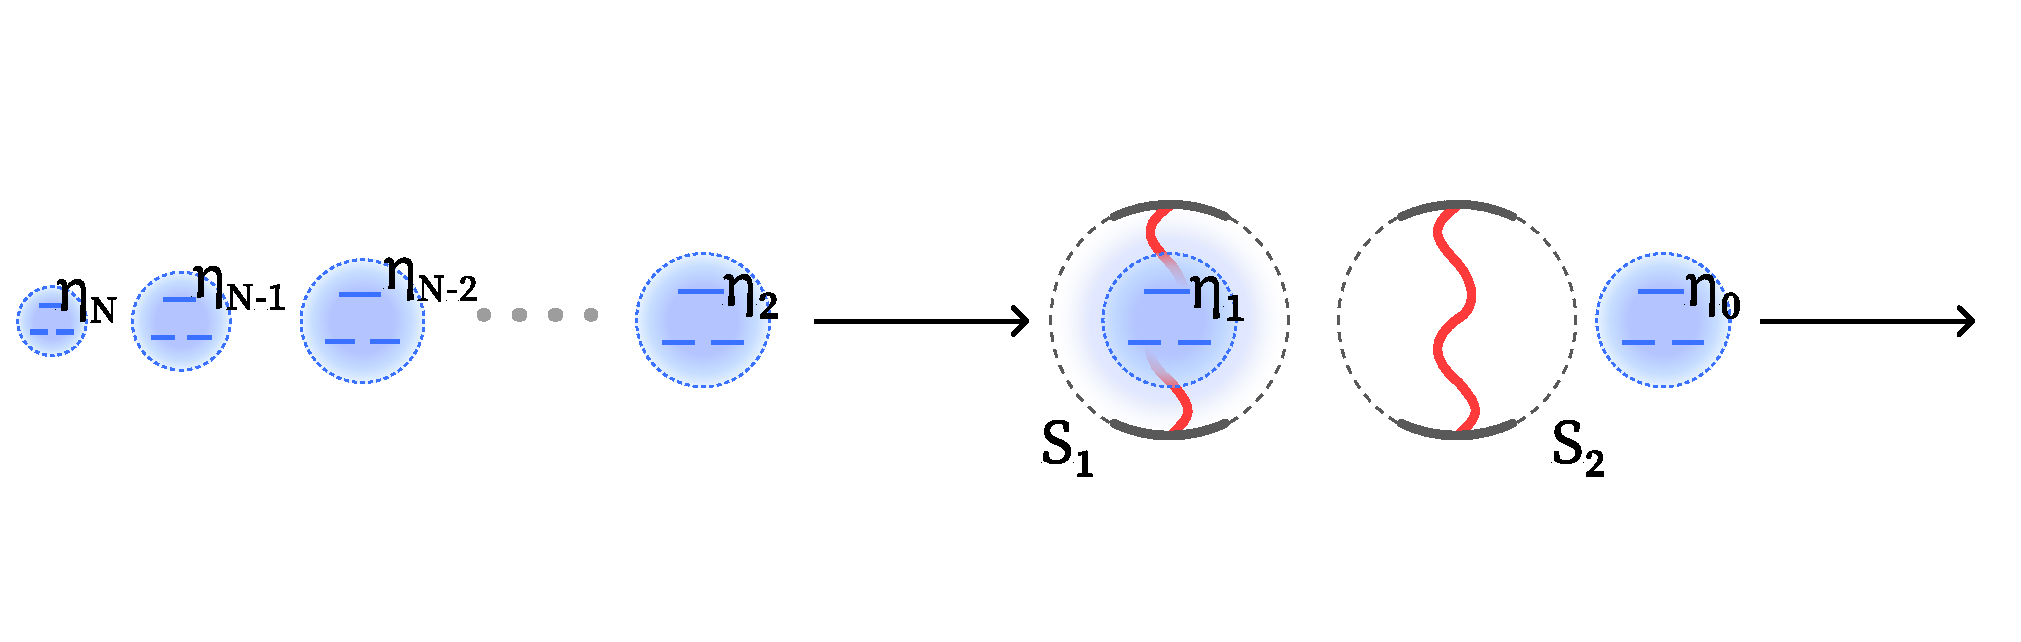
\includegraphics[width=0.9\textwidth]{images/phaseonium_horizontal.pdf}
\caption{ Standard collision model for a phaseonium bath interacting with a multipartite system. The system of interest is a cascade of two single-mode cavity fields $S_1$, $S_2$, which is described by a density operator $\rho$. The environment is made up of $N$ three-level atoms in lambda configuration, called phaseonium atoms, all prepared equally. These atoms play the role of ancillas and are described by a density operator $\eta_k$ ($k=0,\ldots, N$). Ancillas travel at speed $v$ and enter the cavities at a rate $r$. They interact with each cavity field for a time $\Delta t$. The speed and rate of phaseonium atoms is selected such that there is at most one ancilla in each cavity at a time.}
\label{fig:cascade-setup}
\end{figure*}

Each cavity is coupled to the environment via short-time interactions with ancilla systems pumped in the cavity itself. 
Every ancilla $\eta_k\,,k=0,\ldots,N$, is a three-level lambda system. Its states are denoted by $\ket{e}$, $\ket{g_1}$, and $\ket{g_2}$, where $\ket{e}$ represents the excited state while $\ket{g_1}$, $\ket{g_2}$ are two ground states. 
In this basis, the coherent ancilla state which defines the phaseonium \cite{SCULLY1997} can be represented by the density operator
\begin{equation}
\label{def:ancilla-state}
    \eta_k = 
\begin{pmatrix}
\begin{array}{ccc}
    \alpha^2 & 0 & 0
\\
    0 & \frac{\beta^2}{2} & \frac{\beta^2}{2} e^{-i \phi} 
\\[.3em]
    0 & \frac{\beta^2}{2}  e^{i \phi } & \frac{\beta^2}{2} \\
\end{array}
\end{pmatrix}
\,.\end{equation}
with the condition $\abs{\alpha}^2~=~1-\abs{\beta}^2$ to have a unitary trace.
One can thus write a simple free Hamiltonian $\hat{H}_\eta = \hbar\omega_\eta\ket{e}\bra{e}$ for the phaseonium.

We choose a resonant coupling with $\omega_c = \omega_\eta \equiv \omega$ and use the interaction picture to leave the free evolution of both cavity and bath out of the analysis.
So, indicating with $\Omega$ the coupling strength, the total system-environment Hamiltonian at the $k$-th collision is given by the interaction term
\begin{equation}\label{def:interaction}
    \hat{V}_k = \hbar\Omega\left[ \a(\dyad{e}{g_1}+\dyad{e}{g_2}) + \ad(\dyad{g_1}{e}+\dyad{g_2}{e}) \right] \,.
\end{equation}
\\

%%%%%%%%%%%%%%%%%%%%%%%%%%%%%%%%%%%%%%%%%%
\section{Results}
\subsection{One Cavity}
% ============================ %
% FULL-COHERENT PHASEONIUM
\newpage
What is the full dynamics of the system under the interaction with a full-coherent phaseonium $\rho_{n+1}=\Tr\left[U\rho\otimes\eta_{\text{full}}U^\dagger\right]$?

\begin{equation}
    \eta_{\text{full}} = \begin{pmatrix}
        \alpha^2 & \chi_{21} & \chi_{31} \\
        \bar{\chi}_{21} & \frac{\beta^2}{2} & \eta_{32} \\
        \bar{\chi}_{31} & \bar{\eta}_{32} & \frac{\beta^2}{2}  
    \end{pmatrix}
\end{equation}

% CALCULATIONS
%\renewenvironment{imported}
{
% Phaseonium coherences
\newcommand{\chidowntwo}{\bar{\chi}_{31}}
\newcommand{\chidownone}{\bar{\chi}_{21}}
\newcommand{\chiupone}{\chi_{21}}
\newcommand{\chiuptwo}{\chi_{31}}
\newcommand{\etadown}{\bar{\eta}_{32}}
\renewcommand{\etaup}{\eta_{32}}
\renewcommand{\a}{\alpha^2}
\renewcommand{\b}{\frac{\beta^2}{2}}
}
{}

\begin{imported}
The unitary evolution operator is defined as:
\begin{equation}
    e^{i\theta\hat{V}_n} = \begin{pmatrix}
        C & i\Sd & i\Sd \\
        i\S & \frac{\Cp+\idd}{2}& \frac{\Cp-\idd}{2} \\
        i\S & \frac{\Cp-\idd}{2} & \frac{\Cp+\idd}{2}
    \end{pmatrix}
\end{equation}

Tracing out ancilla's degrees of freedom, we have

\begin{align}
    &\rho_{n+1} =
    \left( \a\C\r + i\chidownone\Sd\r + i\chidowntwo\Sd\r \right)\C
    \\ +&
    \left(\etadown\frac{\Cp-\idd}{2}\r + \b\frac{\Cp+\idd}{2}\r +i\chiupone\S\r \right)\frac{\Cp+\idd}{2}
     +
    \left(\etaup\frac{\Cp-\idd}{2}\r + \b\frac{\Cp+\idd}{2}\r +i\chiuptwo\S\r \right)\frac{\Cp+\idd}{2}
    \\ +&
    \left( \b\frac{\Cp-\idd}{2}\r + \etaup\frac{\Cp+\idd}{2}\r + i\chiuptwo\S\r \right)\frac{\Cp-\idd}{2}
    +
    \left( \b\frac{\Cp-\idd}{2}\r + \etadown\frac{\Cp+\idd}{2}\r + i\chiupone\S\r \right)\frac{\Cp-\idd}{2}
    \\ -&
    i\left( \chidowntwo\frac{\Cp-\idd}{2}\r + \chidownone\frac{\Cp+\idd}{2}\r + i\a\S\r \right)\Sd 
    -
    i\left( \chidownone\frac{\Cp-\idd}{2}\r + \chidowntwo\frac{\Cp+\idd}{2}\r + i\a\S\r \right)\Sd 
    \\ -&
    i\left( \chiupone\C\r +i\b\Sd\r +i\etadown\Sd\r \right)\S
    -
    i\left( \chiuptwo\C\r +i\b\Sd\r +i\etaup\Sd\r \right)\S
\end{align}

and so
\begin{align}
    &\rho_{n+1} =
    \left( \a\C\r + i\chidownone\Sd\r + i\chidowntwo\Sd\r \right)\C
    \\ +&
    \frac{1}{2}\left(\etadown\frac{\Cp-\idd}{2}\r + \b\frac{\Cp+\idd}{2}\r +i\chiupone\S\r 
     +
    \etaup\frac{\Cp-\idd}{2}\r + \b\frac{\Cp+\idd}{2}\r +i\chiuptwo\S\r \right)\Cp
    \\ +&
    \frac{1}{2}\left(\etadown\frac{\Cp-\idd}{2}\r + \b\frac{\Cp+\idd}{2}\r +i\chiupone\S\r 
     +
    \etaup\frac{\Cp-\idd}{2}\r + \b\frac{\Cp+\idd}{2}\r +i\chiuptwo\S\r \right)\idd
    \\ +&
    \frac{1}{2}\left( \b\frac{\Cp-\idd}{2}\r + \etaup\frac{\Cp+\idd}{2}\r + i\chiuptwo\S\r
    +
    \b\frac{\Cp-\idd}{2}\r + \etadown\frac{\Cp+\idd}{2}\r + i\chiupone\S\r \right)\Cp
    \\ -&
    \frac{1}{2}\left( \b\frac{\Cp-\idd}{2}\r + \etaup\frac{\Cp+\idd}{2}\r + i\chiuptwo\S\r
    +
    \b\frac{\Cp-\idd}{2}\r + \etadown\frac{\Cp+\idd}{2}\r + i\chiupone\S\r \right)\idd
    \\ -&
    i\left( \chidowntwo\frac{\Cp-\idd}{2}\r + \chidownone\frac{\Cp+\idd}{2}\r + i\a\S\r 
    +
    \chidownone\frac{\Cp-\idd}{2}\r + \chidowntwo\frac{\Cp+\idd}{2}\r + i\a\S\r \right)\Sd 
    \\ -&
    i\left( \chiupone\C\r +i\b\Sd\r +i\etadown\Sd\r 
    +
    \chiuptwo\C\r +i\b\Sd\r +i\etaup\Sd\r \right)\S
\end{align}

\begin{align}
    &\rho_{n+1} =
    \left( \a\C\r + i\chidownone\Sd\r + i\chidowntwo\Sd\r \right)\C
    \\ +&
    \frac{1}{2}\left((\etadown+\etaup)\frac{\Cp-\idd}{2}\r + \beta^2\frac{\Cp+\idd}{2}\r +i(\chiupone+\chiuptwo)\S\r \right)\Cp
    \\ +&
    \frac{1}{2}\left((\etadown+\etaup)\frac{\Cp-\idd}{2}\r + \beta^2\frac{\Cp+\idd}{2}\r +i(\chiupone+\chiuptwo)\S\r \right)\idd
    \\ +&
    \frac{1}{2}\left( \beta^2\frac{\Cp-\idd}{2}\r + (\etadown+\etaup)\frac{\Cp+\idd}{2}\r +i(\chiupone+\chiuptwo)\S\r \right)\Cp
    \\ -&
    \frac{1}{2}\left( \beta^2\frac{\Cp-\idd}{2}\r + (\etadown+\etaup)\frac{\Cp+\idd}{2}\r +i(\chiupone+\chiuptwo)\S\r \right)\idd
    \\ -&
    i\left( (\chidowntwo+\chidownone)\frac{\Cp-\idd}{2}\r + (\chidownone+\chidowntwo)\frac{\Cp+\idd}{2}\r + 2i\a\S\r \right)\Sd 
    \\ -&
    i\left( \chiupone\C\r +i(\beta^2 + \etadown + \etaup)\Sd\r 
    +
    \chiuptwo\C\r \right)\S
\end{align}

\begin{align}
    &\rho_{n+1} =
    \left[ \a\C + i\chidownone\Sd + i\chidowntwo\Sd \right]\r\C
    \\ +&
    \frac{1}{2}\bigg[(\etadown+\etaup)\frac{\Cp-\idd}{2} + \beta^2\frac{\Cp+\idd}{2} +i(\chiupone+\chiuptwo)\S 
    \\ &+
    \beta^2\frac{\Cp-\idd}{2} + (\etadown+\etaup)\frac{\Cp+\idd}{2} +i(\chiupone+\chiuptwo)\S \bigg]\r\Cp
    \\ +&
    \frac{1}{2}\bigg[(\etadown+\etaup)\frac{\Cp-\idd}{2} + \beta^2\frac{\Cp+\idd}{2} +i(\chiupone+\chiuptwo)\S 
    \\ &-
    \beta^2\frac{\Cp-\idd}{2} - (\etadown+\etaup)\frac{\Cp+\idd}{2} -i(\chiupone+\chiuptwo)\S \bigg]\r\idd
    \\ -&
    i\left[ (\chidowntwo+\chidownone)\left(\frac{\Cp-\idd}{2} + \frac{\Cp+\idd}{2}\right) + 2i\a\S \right]\r\Sd 
    \\ -&
    i\left[ \chiupone\C +i(\beta^2 + \etadown + \etaup)\Sd + \chiuptwo\C \right]\r\S
\end{align}

\begin{align}
    &\rho_{n+1} =
    \left[ \a\C + i\chidownone\Sd + i\chidowntwo\Sd \right]\r\C
    \\ +&
    \frac{1}{2}\bigg[\frac{1}{2}\left((\etadown+\etaup) + \beta^2 + \beta^2 + (\etadown+\etaup)\right)\Cp + 2i(\chiupone+\chiuptwo)\S 
    \\ &+
    \frac{1}{2}\left((\etadown+\etaup) + \beta^2 - \beta^2 - (\etadown+\etaup)\right)\idd \bigg]\r\Cp
    \\ +&
    \frac{1}{2}\bigg[\frac{1}{2}\left((\etadown+\etaup)+\beta^2-\beta^2-(\etadown+\etaup)\right)\Cp
    \\ &+
    \frac{1}{2}\left(-(\etadown+\etaup)+\beta^2+\beta^2-(\etadown+\etaup)\right)\idd  \bigg]\r\idd
    \\ -&
    i\left[ (\chidowntwo+\chidownone)\Cp + 2i\a\S \right]\r\Sd 
    \\ -&
    i\left[ \chiupone\C +i(\beta^2 + \etadown + \etaup)\Sd + \chiuptwo\C \right]\r\S
\end{align}

\begin{align}
    &\rho_{n+1} =
    \left[ \a\C + i\chidownone\Sd + i\chidowntwo\Sd \right]\r\C
    \\ +&
    \frac{1}{2}\bigg[\left(\beta^2 + \etadown+\etaup\right)\Cp + 2i(\chiupone+\chiuptwo)\S 
    \bigg]\r\Cp
    \\ +&
    \frac{1}{2}\bigg[\left(\beta^2-\etadown-\etaup\right)\idd  \bigg]\r\idd
    \\ -&
    i\left[ (\chidowntwo+\chidownone)\Cp + 2i\a\S \right]\r\Sd 
    \\ -&
    i\left[ \chiupone\C +i(\beta^2 + \etadown + \etaup)\Sd + \chiuptwo\C \right]\r\S
\end{align}

Now we call $B(\phi)\equiv(\beta^2+\etaup+\etadown)$ and $\bar{B}(\phi)\equiv(\beta^2-\etaup-\etadown)$:

\begin{align}
    \rho_{n+1} =&
    \a\C\r\C 
    +\frac{1}{2}B(\phi)\Cp\r\Cp
    +B(\phi)\Sd\r\S 
    +2\a\S\r\Sd 
    +\frac{1}{2}\bar{B}(\phi)\idd\r\idd
    \\
    &+i(\chidownone+\chidowntwo)(\Sd\r\C - \Cp\r\Sd)
    +i(\chiupone+\chiuptwo)(\S\r\Cp - \C\r\S)
\end{align}

With our previous notation $\etaup = \b e^{-i\phi}$ and $\etadown = \b e^{i\phi}$
\begin{align}
    B(\phi) =& \beta^2+\etaup+\etadown = \beta^2 + \b (e^{-i\phi} + e^{i\phi}) \\
    &\,= \beta^2 (1 + 1/2(\cos\phi -i\sin\phi + \cos\phi +i\sin\phi)) = \beta^2(1+\cos\phi) 
    \\
    \bar{B}(\phi) =& \beta^2-\etaup-\etadown = \beta^2 - \b (e^{-i\phi} + e^{i\phi}) \\
    &\,= \beta^2 (1 - 1/2(\cos\phi -i\sin\phi + \cos\phi +i\sin\phi)) = \beta^2(1 - \cos\phi) 
\end{align}
then $2\alpha^2 = \gamma_\alpha$ and $\beta^2(1+\cos\phi) = \gamma_\beta$.
\\[10pt]


% This is given by Kraus Operators:
%\begin{align}
%    \hat{E}_0 =& \sqrt{\frac{\beta^2}{2}(1-\cos\phi)}\idd \,, \\
%    \hat{E}_1 =& \frac{\sqrt{\ga}}{2}\C \,, \\
%    \hat{E}_2 =& \sqrt{\gamma_\alpha}\Sd \,, \\
%    \hat{E}_3 =& \sqrt{\frac{\gamma_\beta}{2}}\Cp \,, \\
%    \hat{E}_4 =& \sqrt{\gamma_\beta}\S \,,\\
%\end{align}
\end{imported}
\vspace{5pt}

Eventually we find the discrete Master Equation
\begin{equation}\label{eq:full-coherent-map}
\begin{split}
    \rho_{n+1} =&
    \alpha^2\C\rho_n\C 
    +2\alpha^2\S\rho_n\Sd 
    +\frac{\beta^2}{2}(1+\cos\phi)\Cp\rho_n\Cp
    +\beta^2(1+\cos\phi)\Sd\rho_n\S 
    +\frac{\beta^2}{2}(1 - \cos\phi)\idd\rho_n\idd
    \\
    &+i(\bar{\chi}_{21}+\bar{\chi}_{31})(\Sd\rho_n\C - \Cp\rho_n\Sd)
    +i(\chi_{21}+\chi_{31})(\S\rho_n\Cp - \C\rho_n\S)
\end{split}
\end{equation}
where the first line is equal to our known Kraus map.


\section{Continuous Times}
% ========================== %
For short-time approximation, photonic operators in Eq.~\cref{eq:full-coherent-map} become
\begin{equation}\label{eq:short-time-approx}
    %&\equiv \cos(\theta\sqrt{2aa^\dagger}) \rightarrow
    C=\mathbb{I} - \theta^2aa^\dagger \qquad
    %\cos(\theta\sqrt{2a^\dagger a}) 
    C'= \mathbb{I} - \theta^2a^\dagger a \qquad
    % a^\dagger \frac{\sin(\theta\sqrt{2aa^\dagger})}{\sqrt{2aa^\dagger}} 
    S = \theta a^\dagger 
\end{equation}

% CALCULATIONS
%\renewenvironment{imported}{
% Local new commands here
% \newcommand{}{}
}
{}


Neglecting terms of the order $\Delta t^3$ ($\theta^3$) and higher we have:

\begin{align}
    \rho_{n+1} =&
    \alpha^2\left(\r - \tt\r\a\ad - \tt\a\ad\r \right)
    +2\alpha^2\left( \tt\ad\r\a \right)\\
    &+\frac{\beta^2}{2}(1+\cos\phi)\left( \r -\tt\r\ad\a -\tt\ad\a\r \right)   +\beta^2(1+\cos\phi)\left( \tt\a\r\ad \right) \\
    &+i(\bar{\chi}_{21}+\bar{\chi}_{31})(\theta\a\r\idd - \theta\idd\r\a) \\
    &+i(\chi_{21}+\chi_{31})(\theta\ad\r\idd - \theta\idd\r\ad) \\
    &+\frac{\beta^2}{2}(1 - \cos\phi)\r
\end{align}
and so
\begin{align}
    \rho_{n+1} =&
    \alpha^2\left( - \tt\r\a\ad - \tt\a\ad\r 
    +2\tt\ad\r\a \right) +\alpha^2\r \\
    &+\frac{\beta^2}{2}(1+\cos\phi)\left( -\tt\r\ad\a -\tt\ad\a\r + 2\tt\a\r\ad \right) +\frac{\beta^2}{2}(1+\cos\phi)\r\\
    &+i\theta(\bar{\chi}_{21}+\bar{\chi}_{31})(\a\r - \r\a) \\
    &+i\theta(\chi_{21}+\chi_{31})(\ad\r - \r\ad) \\
    &+\frac{\beta^2}{2}(1 - \cos\phi)\r
\end{align}
and this is
\begin{align}
    \rho_{n+1} =&
    2\alpha^2\tt\left(\ad\r\a -\frac{1}{2}\acomm{\a\ad}{\r} \right) \\
    &+\beta^2(1+\cos\phi)\tt\left(\a\r\ad -\frac{1}{2}\acomm{\ad\a}{\r} \right) \\
    &+i\theta\comm{(\bar{\chi}_{21}+\bar{\chi}_{31})\a + (\chi_{21}+\chi_{31})\ad}{\r} \\
    &+\left( \alpha^2 +\frac{\beta^2}{2}(1+\cos\phi) + \frac{\beta^2}{2}(1 - \cos\phi) \right)\r
\end{align}

The final form of the master equation is:
\begin{equation}
\begin{split}
    \frac{\rho_{n+1} - \rho_n}{\Delta t} =
    +&i\comm{\hbar\Omega H_{\text{work}}}{\r} \\
    +&\ga(\hbar\Omega)^2\Delta t\left(\ad\rho_n\a -\frac{1}{2}\acomm{\a\ad}{\rho_n} \right)
    +\gb(\hbar\Omega)^2\Delta t\left(\a\rho_n\ad -\frac{1}{2}\acomm{\ad\a}{\rho_n} \right) 
\end{split}
\end{equation}
with $H_{\text{work}}\equiv(\bar{\chi}_{21}+\bar{\chi}_{31})\a + (\chi_{21}+\chi_{31})\ad$.

\subsection{Two Cavities}
\renewcommand{\b}{\hat{b}}
With the short-time approximation in Eq.~\ref{eq:short-time-approx}, denoting $\a$ ( $\ad$ ) and $\hat{b}$ ($\bd$) as the annihilation (creation) operators for the first  and second cavity respectively, the Kraus operators in \ref{def:kraus2} can be written as
%We can thus drop the tensor product symbol $\otimes$.
%Approximating to second-order terms in $\theta$, we have
\begin{align}
    E_0 &= \sqrt{1-\frac{\gamma_\alpha}{2}-\frac{\gamma_\beta}{2}}\mathbb{I}\, , 
    \\[1em]
    E_1 &= \sqrt{\frac{\gamma_\alpha}{2}}\left[ 1-\tt\b\bd-\tt\a\ad-2\tt\ad\b \right]\, ,
    \\[1em]
    E_2 &= \sqrt{\gamma_\alpha}\left[ \theta\ad + \theta\bd \right]\, ,
    \\[1em]
    E_3 &= \sqrt{\gamma_\beta}\left[ \theta\a + \theta\b \right]\, ,
    \\[1em]
    E_4 &= \sqrt{\frac{\gamma_\beta}{2}}\left[ 1-\tt\bd\b-\tt\ad\a-2\tt\a\bd \right]\, ,
\end{align}
where $\ga=2\alpha^2$ and $\gb=\beta^2(1+\cos\phi)$.

We can now use these expressions to rewrite the discrete master equation
(\ref{eq:finitediff_ME}) as
\begin{align}\label{def:lindbladian-evolution}
    \frac{d\rho(t)}{d t}
    %= &\mathcal{L}\hat{\rho}(t)\\
    = -i[\hat{H}_\text{eff},\rho] +  \gamma'_\alpha \,\mathcal{D}[\hat{a}^\dagger{+}\hat{b}^\dagger]\,\hat{\rho}(t)+\gamma'_\beta \,\mathcal{D}[\hat{a}{+}\hat{b}]\,\hat{\rho}(t)
\end{align}

where $\hat{H}_\text{eff}=i(\gamma'_\beta-\gamma'_\alpha)(\ad \b-\bd\a)/2$ and $\gamma'_{\alpha,\beta}=\gamma_{\alpha,\beta}\Omega^2\Delta t$, considering always $\Omega$ such that $\Omega^2 \Delta t$ converges in the continuous limit.

We now derive the master equation describing the dynamics of the two cavities in the case in which are present coherence also between the excited and the two ground states of the phaseonium bath. 

In this case $\rho_n \in \mathcal{H}_1\otimes\mathcal{H}_2$ and $\sigma_n=\rho_n\otimes\eta$, so the evolution is described by
\begin{equation}
\sigma_{n+1}=U_2 U_1\sigma_n U^\dagger_1 U^\dagger_2
\end{equation}

Taking the continuous limit, i.e. taking $U_i$ up to the second order,

\begin{multline}
\sigma_{n+1}=(\mathbb{I}-i\theta V_2-\frac{\theta^2}{2} V^2_2)(\mathbb{I}-i\theta V_1-\frac{\theta^2}{2} V^2_1)\sigma_n(\mathbb{I}+i\theta V_1-\frac{\theta^2}{2} V^2_1)(\mathbb{I}+i\theta V_2-\frac{\theta^2}{2} V^2_2)=\\
=(\mathbb{I}-i\theta V_2-i\theta V_1-\frac{\theta^2}{2} V^2_2-\frac{\theta^2}{2} V^2_1-\theta^2V_2V_1)\sigma_n(\mathbb{I}+i\theta V_2+i\theta V_1-\frac{\theta^2}{2} V^2_2-\frac{\theta^2}{2} V^2_1-\theta^2V_1V_2)=\\
=\sigma_n-i\theta[V_2,\sigma_n]-i\theta[V_1,\sigma_n]+\theta^2V_1\sigma_nV_2+\theta^2V_2\sigma_nV_1+\\+\theta^2(V_1\sigma_nV_1-\frac{1}{2}[V^2_1,\sigma_n]_+)+\theta^2(V_2\sigma_nV_2-\frac{1}{2}[V^2_2,\sigma_n]_+)-\theta^2V_2V_1\sigma_n-\theta^2V_1V_2\sigma_n
\end{multline}

Taking the difference between the ($n+1$)-th step and the n-th step, dividing by $\theta$ and tracing out the degrees of freedom one obtains \eqref{def:lindbladian-evolution}, but in this case $\hat{H}_\text{eff}=i(\gamma'_\beta-\gamma'_\alpha)(\a\b-\bd\a)/2+((\bar{\chi}_{21}+\bar{\chi}_{31})(\a+\b)+(\chi_{21}+\chi_{31})(\ad+\bd) )$



%%%%%%%%%%%%%%%%%%%%%%%%%%%%%%%%%%%%%%%%%%
\section{Discussion}

Authors should discuss the results and how they can be interpreted from the perspective of previous studies and of the working hypotheses. The findings and their implications should be discussed in the broadest context possible. Future research directions may also be highlighted.

%%%%%%%%%%%%%%%%%%%%%%%%%%%%%%%%%%%%%%%%%%
\section{Conclusions}

This section is not mandatory, but can be added to the manuscript if the discussion is unusually long or complex.


%%%%%%%%%%%%%%%%%%%%%%%%%%%%%%%%%%%%%%%%%%
\vspace{6pt} 

%%%%%%%%%%%%%%%%%%%%%%%%%%%%%%%%%%%%%%%%%%
%% optional
%\supplementary{The following supporting information can be downloaded at:  \linksupplementary{s1}, Figure S1: title; Table S1: title; Video S1: title.}

% Only for journal Methods and Protocols:
% If you wish to submit a video article, please do so with any other supplementary material.
% \supplementary{The following supporting information can be downloaded at: \linksupplementary{s1}, Figure S1: title; Table S1: title; Video S1: title. A supporting video article is available at doi: link.}

% Only for journal Hardware:
% If you wish to submit a video article, please do so with any other supplementary material.
% \supplementary{The following supporting information can be downloaded at: \linksupplementary{s1}, Figure S1: title; Table S1: title; Video S1: title.\vspace{6pt}\\
%\begin{tabularx}{\textwidth}{lll}
%\toprule
%\textbf{Name} & \textbf{Type} & \textbf{Description} \\
%\midrule
%S1 & Python script (.py) & Script of python source code used in XX \\
%S2 & Text (.txt) & Script of modelling code used to make Figure X \\
%S3 & Text (.txt) & Raw data from experiment X \\
%S4 & Video (.mp4) & Video demonstrating the hardware in use \\
%... & ... & ... \\
%\bottomrule
%\end{tabularx}
%}

%%%%%%%%%%%%%%%%%%%%%%%%%%%%%%%%%%%%%%%%%%
\authorcontributions{For research articles with several authors, a short paragraph specifying their individual contributions must be provided. The following statements should be used ``Conceptualization, X.X. and Y.Y.; methodology, X.X.; software, X.X.; validation, X.X., Y.Y. and Z.Z.; formal analysis, X.X.; investigation, X.X.; resources, X.X.; data curation, X.X.; writing---original draft preparation, X.X.; writing---review and editing, X.X.; visualization, X.X.; supervision, X.X.; project administration, X.X.; funding acquisition, Y.Y. All authors have read and agreed to the published version of the manuscript.'', please turn to the  \href{http://img.mdpi.org/data/contributor-role-instruction.pdf}{CRediT taxonomy} for the term explanation. Authorship must be limited to those who have contributed substantially to the work~reported.}

\funding{Please add: ``This research received no external funding'' or ``This research was funded by NAME OF FUNDER grant number XXX.'' and  and ``The APC was funded by XXX''. Check carefully that the details given are accurate and use the standard spelling of funding agency names at \url{https://search.crossref.org/funding}, any errors may affect your future funding.}

\institutionalreview{In this section, you should add the Institutional Review Board Statement and approval number, if relevant to your study. You might choose to exclude this statement if the study did not require ethical approval. Please note that the Editorial Office might ask you for further information. Please add “The study was conducted in accordance with the Declaration of Helsinki, and approved by the Institutional Review Board (or Ethics Committee) of NAME OF INSTITUTE (protocol code XXX and date of approval).” for studies involving humans. OR “The animal study protocol was approved by the Institutional Review Board (or Ethics Committee) of NAME OF INSTITUTE (protocol code XXX and date of approval).” for studies involving animals. OR “Ethical review and approval were waived for this study due to REASON (please provide a detailed justification).” OR “Not applicable” for studies not involving humans or animals.}

\informedconsent{Any research article describing a study involving humans should contain this statement. Please add ``Informed consent was obtained from all subjects involved in the study.'' OR ``Patient consent was waived due to REASON (please provide a detailed justification).'' OR ``Not applicable'' for studies not involving humans. You might also choose to exclude this statement if the study did not involve humans.

Written informed consent for publication must be obtained from participating patients who can be identified (including by the patients themselves). Please state ``Written informed consent has been obtained from the patient(s) to publish this paper'' if applicable.}

\dataavailability{We encourage all authors of articles published in MDPI journals to share their research data. In this section, please provide details regarding where data supporting reported results can be found, including links to publicly archived datasets analyzed or generated during the study. Where no new data were created, or where data is unavailable due to privacy or ethical restrictions, a statement is still required. Suggested Data Availability Statements are available in section ``MDPI Research Data Policies'' at \url{https://www.mdpi.com/ethics}.} 

% Only for journal Nursing Reports
%\publicinvolvement{Please describe how the public (patients, consumers, carers) were involved in the research. Consider reporting against the GRIPP2 (Guidance for Reporting Involvement of Patients and the Public) checklist. If the public were not involved in any aspect of the research add: ``No public involvement in any aspect of this research''.}

% Only for journal Nursing Reports
%\guidelinesstandards{Please add a statement indicating which reporting guideline was used when drafting the report. For example, ``This manuscript was drafted against the XXX (the full name of reporting guidelines and citation) for XXX (type of research) research''. A complete list of reporting guidelines can be accessed via the equator network: \url{https://www.equator-network.org/}.}

\acknowledgments{In this section you can acknowledge any support given which is not covered by the author contribution or funding sections. This may include administrative and technical support, or donations in kind (e.g., materials used for experiments).}

\conflictsofinterest{Declare conflicts of interest or state ``The authors declare no conflicts of interest.'' Authors must identify and declare any personal circumstances or interest that may be perceived as inappropriately influencing the representation or interpretation of reported research results. Any role of the funders in the design of the study; in the collection, analyses or interpretation of data; in the writing of the manuscript; or in the decision to publish the results must be declared in this section. If there is no role, please state ``The funders had no role in the design of the study; in the collection, analyses, or interpretation of data; in the writing of the manuscript; or in the decision to publish the results''.} 

%%%%%%%%%%%%%%%%%%%%%%%%%%%%%%%%%%%%%%%%%%
%% Optional

\abbreviations{Abbreviations}{
The following abbreviations are used in this manuscript:\\

\noindent 
\begin{tabular}{@{}ll}
MDPI & Multidisciplinary Digital Publishing Institute\\
DOAJ & Directory of open access journals\\
TLA & Three letter acronym\\
LD & Linear dichroism
\end{tabular}
}

%%%%%%%%%%%%%%%%%%%%%%%%%%%%%%%%%%%%%%%%%%
%% Optional
\appendixtitles{no} % Leave argument "no" if all appendix headings stay EMPTY (then no dot is printed after "Appendix A"). If the appendix sections contain a heading then change the argument to "yes".
\appendixstart
\appendix
\section[\appendixname~\thesection]{}
\subsection[\appendixname~\thesubsection]{}
The appendix is an optional section that can contain details and data supplemental to the main text---for example, explanations of experimental details that would disrupt the flow of the main text but nonetheless remain crucial to understanding and reproducing the research shown; figures of replicates for experiments of which representative data are shown in the main text can be added here if brief, or as Supplementary Data. Mathematical proofs of results not central to the paper can be added as an appendix.

\begin{table}[H] 
\caption{This is a table caption.\label{tab5}}
\newcolumntype{C}{>{\centering\arraybackslash}X}
\begin{tabularx}{\textwidth}{CCC}
\toprule
\textbf{Title 1}	& \textbf{Title 2}	& \textbf{Title 3}\\
\midrule
Entry 1		& Data			& Data\\
Entry 2		& Data			& Data\\
\bottomrule
\end{tabularx}
\end{table}

\section[\appendixname~\thesection]{}
All appendix sections must be cited in the main text. In the appendices, Figures, Tables, etc. should be labeled, starting with ``A''---e.g., Figure A1, Figure A2, etc.

%%%%%%%%%%%%%%%%%%%%%%%%%%%%%%%%%%%%%%%%%%
\begin{adjustwidth}{-\extralength}{0cm}
%\printendnotes[custom] % Un-comment to print a list of endnotes

\reftitle{References}

% Please provide either the correct journal abbreviation (e.g. according to the “List of Title Word Abbreviations” http://www.issn.org/services/online-services/access-to-the-ltwa/) or the full name of the journal.
% Citations and References in Supplementary files are permitted provided that they also appear in the reference list here. 

%=====================================
% References, variant A: external bibliography
%=====================================
%\bibliography{your_external_BibTeX_file}

%=====================================
% References, variant B: internal bibliography
%=====================================
\begin{thebibliography}{999}
% Reference 1
\bibitem[Author1(year)]{ref-journal}
Author~1, T. The title of the cited article. {\em Journal Abbreviation} {\bf 2008}, {\em 10}, 142--149.
% Reference 2
\bibitem[Author2(year)]{ref-book1}
Author~2, L. The title of the cited contribution. In {\em The Book Title}; Editor 1, F., Editor 2, A., Eds.; Publishing House: City, Country, 2007; pp. 32--58.
% Reference 3
\bibitem[Author3(year)]{ref-book2}
Author 1, A.; Author 2, B. \textit{Book Title}, 3rd ed.; Publisher: Publisher Location, Country, 2008; pp. 154--196.
% Reference 4
\bibitem[Author4(year)]{ref-unpublish}
Author 1, A.B.; Author 2, C. Title of Unpublished Work. \textit{Abbreviated Journal Name} year, \textit{phrase indicating stage of publication (submitted; accepted; in press)}.
% Reference 5
\bibitem[Author5(year)]{ref-communication}
Author 1, A.B. (University, City, State, Country); Author 2, C. (Institute, City, State, Country). Personal communication, 2012.
% Reference 6
\bibitem[Author6(year)]{ref-proceeding}
Author 1, A.B.; Author 2, C.D.; Author 3, E.F. Title of presentation. In Proceedings of the Name of the Conference, Location of Conference, Country, Date of Conference (Day Month Year); Abstract Number (optional), Pagination (optional).
% Reference 7
\bibitem[Author7(year)]{ref-thesis}
Author 1, A.B. Title of Thesis. Level of Thesis, Degree-Granting University, Location of University, Date of Completion.
% Reference 8
\bibitem[Author8(year)]{ref-url}
Title of Site. Available online: URL (accessed on Day Month Year).
\end{thebibliography}

% If authors have biography, please use the format below
%\section*{Short Biography of Authors}
%\bio
%{\raisebox{-0.35cm}{\includegraphics[width=3.5cm,height=5.3cm,clip,keepaspectratio]{Definitions/author1.pdf}}}
%{\textbf{Firstname Lastname} Biography of first author}
%
%\bio
%{\raisebox{-0.35cm}{\includegraphics[width=3.5cm,height=5.3cm,clip,keepaspectratio]{Definitions/author2.jpg}}}
%{\textbf{Firstname Lastname} Biography of second author}

% For the MDPI journals use author-date citation, please follow the formatting guidelines on http://www.mdpi.com/authors/references
% To cite two works by the same author: \citeauthor{ref-journal-1a} (\citeyear{ref-journal-1a}, \citeyear{ref-journal-1b}). This produces: Whittaker (1967, 1975)
% To cite two works by the same author with specific pages: \citeauthor{ref-journal-3a} (\citeyear{ref-journal-3a}, p. 328; \citeyear{ref-journal-3b}, p.475). This produces: Wong (1999, p. 328; 2000, p. 475)

%%%%%%%%%%%%%%%%%%%%%%%%%%%%%%%%%%%%%%%%%%
%% for journal Sci
%\reviewreports{\\
%Reviewer 1 comments and authors’ response\\
%Reviewer 2 comments and authors’ response\\
%Reviewer 3 comments and authors’ response
%}
%%%%%%%%%%%%%%%%%%%%%%%%%%%%%%%%%%%%%%%%%%
\PublishersNote{}
\end{adjustwidth}
\end{document}

